
\chapter{Label Propagation}
\label{ch:label-propagation}

Web browsers which execute JavaScript code allow pages to load JavaScript and HTML code from many different sources into the same execution context.
This work distinguishes between JavaScript programs by tagging each with a different label representing its domain of origin.
Many web pages using this technique contain cooperating functions which generate shared objects.
Each object created or modified via the confluence of separate scripts bears a label which tracks all domains influencing the object.

\begin{figure}[ht]
  \centerline{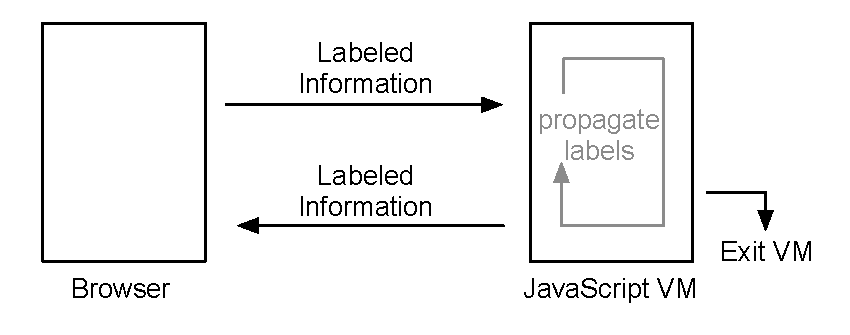
\includegraphics[keepaspectratio=true]{images/browserinteraction.pdf}}
  \caption{Interaction of the browser and the JavaScript~VM}
  \label{fig:browserinteraction}
\end{figure}

\autoref{fig:browserinteraction} illustrates the interaction between the browser and the JavaScript engine.
Before the browser hands a script and its input data to the JavaScript VM, it first labels the script to indicate the domain of origin.
The VM then compiles the script source into an internal bytecode instruction representation.
During this process, static analysis enables the instrumentation of additional instructions (\autoref{ch:instructions}) that allow information flow tracking during execution.

\section{Label Lattice}
\label{sec:label-lattice}

Within the JavaScript VM, data and objects originating from different domains may interact, creating values that are influenced by multiple domains.
To model this behavior, we take inspiration from Myers' decentralized label model~\cite{myers.liskov+00} and represent security labels as a lattice join over domains.
Each web domain corresponds to a separate security principal, shown in the bottom row of \autoref{fig:label-lattice}.

The information flow framework extends JavaScriptCore with a \FlowLabelRegistry\ which maps security principals (web domain name strings) to unique bit positions within the label portion of a \jsvalue.
Taken as a whole, these bit positions form a bit vector that acts as a confidentiality label, holding up to 16~different domains.
This configuration allows labels to represent any element within the lattice over web domains.
\autoref{fig:label-lattice} depicts an example lattice for a page pulling JavaScript programs from three separate domains.

\tikzset{arrow/.style={
  decoration={markings,mark=at position 1 with {\arrow[scale=2.5]{latex'}}},
  postaction={decorate},
  shorten >= 0.4pt}
}

\tikzset{labarrow/.style={
  decoration={markings,
              mark=at position 0 with {\arrow[scale=1.5]{|};},
              mark=at position 1 with {\arrow[scale=2.5]{latex'};}
             },
  postaction={decorate},
  }
}

\tikzset{labelprop/.style={
  decoration={markings,mark=at position 1 with {\arrow[scale=2.5]{latex'}}},
  postaction={decorate},
  shorten >= 0.4pt}
}

\begin{figure}[ht]
\begin{tikzpicture}[node distance = 1cm, auto,
    force/.style={rectangle, inner sep=5pt, text badly centered, minimum height=.8cm}
    ]

    \begin{scope}[yshift=3.75cm, xshift=-7cm]
    \node[shape=rectangle, draw] {
       \begin{tabular}{l|c}
          \multicolumn{2}{c}{\FlowLabelRegistry\ mapping} \\
          \hline
          example.com & \texttt{0001} \\
          maps.com & \texttt{0010} \\
          ad.com & \texttt{0100} \\
       \end{tabular}
    };
    \end{scope}

    \begin{scope}
    \matrix[nodes={force}, column sep=1cm] {
        \node (ex) {example.com}; &
        \node (mp) {maps.com}; &
        \node (ad) {ad.com}; \\
    };
    \end{scope}

    \begin{scope}[yshift=2cm]
    \matrix[nodes={force}, column sep=.5cm] {
      \node (exUmp) {example.com $\sqcup$ maps.com}; &
      \node (exUad) {example.com $\sqcup$ ad.com}; &
      \node (mpUad) {maps.com $\sqcup$ ad.com}; \\
    };
    \end{scope}

    \begin{scope}[yshift=4cm]
    \matrix[nodes={force}, column sep=1cm] {
      \node (exUmpUad) {example.com $\sqcup$ maps.com $\sqcup$ ad.com}; \\
    };
    \end{scope}

    \draw[arrow] (ex) -- (exUmp);
    \draw[arrow] (ex) -- (exUad);

    \draw[arrow] (mp) -- (exUmp);
    \draw[arrow] (mp) -- (mpUad);

    \draw[arrow] (ad) -- (exUad);
    \draw[arrow] (ad) -- (mpUad);

    \draw[arrow] (exUmp) -- (exUmpUad);
    \draw[arrow] (exUad) -- (exUmpUad);
    \draw[arrow] (mpUad) -- (exUmpUad);

\end{tikzpicture}
  \caption{Interaction of the browser and the JavaScript~VM}
  \label{fig:label-lattice}
\end{figure}

Throughout execution, the modified JavaScript VM attaches the security labels to new JavaScript values based on the current execution context and web domain of origin.
Because labels can represent any element from the lattice, the interpreter fully tracks which domains influence each object.

\subsection{Encoding Labels}\label{sec:jitflow-labelencoding}

As a modified version of JavaScriptCore, the \FlowCore\ interpreter already achieves high performance by using a type-tagged union, called \jsvalue, to represent immediate values, object references, and numbers.
In developing \JitFlow, we considered doubling JavaScriptCore's \jsvalue\ type to include an additional 64 bits for storing the security label (\autoref{sec:fat-values}), but decided against that option.
Rather than extending the size of the \JSValue\ data type, it repurposes 16 of the bits to hold the security label.
This modification allows for a low performance overhead encoding that packs both the label and the typed value within the same 64~bit word, avoiding a change to any offset and layout calculations in the JIT compiler.

\begin{figure}[ht]
  \centering
\begin{tabular}{cccc|l}
    \multicolumn{4}{c|}{bit values} & type  \\
\hline
    \code{0000} & \code{xxxx} & \code{pppp} & \code{ppp0} & \code{pointer} \\
\hline
    \code{0000} & \code{xxxx} & \code{0000} & \code{0000} & \code{empty} \\
    \code{0000} & \code{xxxx} & \code{0000} & \code{0002} & \code{null} \\
    \code{0000} & \code{xxxx} & \code{0000} & \code{0004} & \code{deleted} \\
    \code{0000} & \code{xxxx} & \code{0000} & \code{0006} & \code{false} \\
    \code{0000} & \code{xxxx} & \code{0000} & \code{0007} & \code{true} \\
    \code{0000} & \code{xxxx} & \code{0000} & \code{000a} & \code{undefined} \\
\hline
    \code{FFFF} & \code{xxxx} & \code{iiii} & \code{iiii} & \code{integer} \\
\hline
    \code{0001} & \code{dddd} & \code{dddd} & \code{dddd} & \tikzmark{2nd} \multirow{3}{*}{\code{  double}} \\
    \code{\vdots} & & & & \\
    \code{FFFE} & \code{dddd} & \code{dddd} & \code{dddd} & \tikzmark{4th} \\
\hline
     \tikzmark{p1}\code{~~~}\tikzmark{p2} & \tikzmark{p3}\code{~~~}\tikzmark{p4} & \tikzmark{p5}\code{~~~}\tikzmark{p6} & \multicolumn{1}{c}{\tikzmark{p7}\code{~~~}\tikzmark{p8}} & \multicolumn{1}{l}{\tikzmark{p9}} \\
     & & \tikzmark{v1}\code{~~~~} & \multicolumn{1}{c}{\code{~~~~}\tikzmark{v2}} & \multicolumn{1}{l}{} \\
     & \tikzmark{l1}\code{~~~~}\tikzmark{l2} & \multicolumn{2}{c}{} \\
     \tikzmark{t1}\code{~~~~}\tikzmark{t2} & \multicolumn{3}{c}{} \\
\end{tabular}
\begin{tikzpicture}[overlay, remember picture]
    \draw [decoration={brace,amplitude=.5em}, decorate]
    ($(2nd)+(0,1ex)$) -- ($(4th)+(0,1ex)$);

    \draw [|-|] ($(v1)$) -- ($(v2)$) node[anchor=west]{Value};
    \draw [|-|] ($(l1)$) -- ($(l2)$) node[anchor=west]{Label Encoding};
    \draw [|-|] ($(t1)$) -- ($(t2)$) node[anchor=west]{Type Information Tag};
    \node [font=\tiny] at ($(p1)$) {63};
    \node [font=\tiny] at ($(p2)$) {48};
    \node [font=\tiny] at ($(p3)$) {47};
    \node [font=\tiny] at ($(p4)$) {32};
    \node [font=\tiny] at ($(p5)$) {31};
    \node [font=\tiny] at ($(p6)$) {16};
    \node [font=\tiny] at ($(p7)$) {15};
    \node [font=\tiny] at ($(p8)$) {0};
    \node [anchor=west, font=\tiny] at ($(p9)$) {bit position};
\end{tikzpicture}
\caption{
   \label{fig:jitflow-bit-encoding}
   Label encoding using bits 32--47 of \jsvalues, supporting 16 security principals.
}
\end{figure}

Because the repurposing of bits affects the interpretation of the \jsvalue, it pays to examine each case:

\begin{description}

\item[Pointers/Immediates:]
\jsvalues\ starting with the highest 16~bits all set to~zero (\autoref{fig:jitflow-bit-encoding}) indicate either a pointer or immediate type.
The VM uses the lowest four bits to distinguish pointers from immediates.
Pointers have alignment with these bits all set to~zero, while immediate values hold non-zero entries in the same lowest four bits: \code{empty:0x00}, \code{null:0x02}, \code{deleted:0x04}, \code{false:0x06}, \code{true:0x07}, and \code{undefined:0x0a}.

\item[Pointers:]
In JavaScriptCore, pointer addresses occupy 46~bits (bits 0--47).
Unfortunately, this design does not leave any space to directly encode a label within \jsvalues.
Hence, \JitFlow\ modifies allocation of the garbage-collected heap so that it fits within a 32~bit address space.
This change limits the heap to be 4GB in size, but frees 16 bits of JavaScript object references for a security label (bits~32--47, marked as \code{xxxx} in \autoref{fig:jitflow-bit-encoding}).
This modification also permits efficient bit arithmetic for the frequent label join operation, an essential implementation detail for performance when propagating information flow.
At the expense of maximum heap size, \JitFlow\ gains an efficient labeling of virtual machine values.

\item[Integers:]
Values starting with the highest 16~bits all set to~one indicate an integer value type.
ECMAScript~\cite{ecma} specifies that the JavaScript operators only deal with 31~bit integers, leaving bits 32--47 unused by the original JavaScriptCore encoding.
This arrangement means that same set of bits as used previously in pointers and immediates remain free for encoding a label on integers.

\item[Doubles:]
Doubles in the ECMAScript specification follow the double-precision 64~bit format as specified in the IEEE Standard for Binary Floating-Point arithmetic~\cite{ieee754}.
Therefore, JavaScriptCore reserves all values with highest 16~bits between \code{0x0001} and \code{0xfffe} for doubles.
Unfortunately, this encoding uses all available bits for the double value, leaving no room for a label.
To compensate for this shortcoming, \JitFlow\ treats doubles conservatively by implicitly tagging them with the highest security label in the lattice.
This decision makes double values a source of label creep (\autoref{sec:label-creep}).

\end{description}

%------------------------------------------------------------------------------------------------------

\section{Label Operations}

The design decision to use a bit position encoding for web domains limits the framework to at most 16 domains.
Testing with a webcrawler (\autoref{sec:realworldapplicability}) revealed that none of the pages within the Alexa Top 1000~\cite{alexa} had pages that include content from more than 15 different domains.
The framework contains no fundamental design flaws that would prevent an extension to the label encoding.
If necessary, \JitFlow\ could reserve the highest bit in the label field as an overflow, indicating that the page includes content from more than 16 different domains.

\begin{definition}
  Given two security labels, $a$ and $b$, the {\bf join}, $a \sqcup b$, contains security principals that belong to the label $a$, the label $b$, or both.
\end{definition}

Using a bitwise representation allows the use of efficient bit arithmetic for computing the join (bitwise or) of two labels.
This operation occurs in every method call, assignment, and expression evaluation.
For example, when the program adds two numbers, the information flow framework labels the result with the join of the labels of the arguments and the label of the program counter.
Web applications today contain large amounts of JavaScript, which users expect to run without delay.
Label joining occurs frequently enough that any implementation other than bit arithmetic unacceptably penalizes the JavaScript runtime speed.

\begin{definition}
  Given two security labels, $a$ and $b$, the {\bf subsumes} relation, $a \sqsubseteq b$, is true if and only if the set of security principles comprising label $a$ is subset of the security principles comprising label $b$.
\end{definition}

The browser detects information leaks by comparing the label attached to a network request and the destination domain.
To assist with this task, labels support a subsumes relation that reveals the partial order of labels in the lattice.
If the label on the request contains principles other than the destination domain, the browser flags the request as a potential information leak.

\begin{definition}
  Given a security labels $a$ and $b$, the information flow VM {\bf upgrades} label $a$ with $b$ when it replaces $a$ with the join of $a$ and $b$, written $a \gets a \sqcup b$.
\end{definition}

When the Vm assigns value to an existing variable, it upgrades the label on the destination variable with the label attached to the source value.
Because assignment represents a mutation of memory, the VM also upgrades the destination label with the current \pclabel.
The labels faithfully record the dependence of the assignment on the current security context.

%TODO: include equal relation?
%TODO: include strict subsumption?

\section{Control Flow Stack}
\label{sec:control-flow-stack}

In a dynamically typed language such as JavaScript, we cannot apply the techniques of static analysis that rely upon static typing (developed in languages such as Jif~\cite{jif}).
As a result, the information flow modifications to the JavaScriptCore perform tracking up to active implicit information flows.
By handing back label information on values used in construction of a network resource request, the VM modifications increase the data available to the browser for making network policy enforcement decisions.
However, to prevent information leak to third parties, the browser ultimately remains responsible for enforcing a security policy on network traffic.

The syntax of JavaScript programs allows for points where the control flow branches due to the evaluation of a runtime conditional.
At each of these points, the security context of any code executed within the taken branch needs to reflect its dependence on the conditional.
To accomplish this task, we augment the JavaScript interpreter with a stack of labels, called the \term{control flow stack}.
As shown in \autoref{fig:cf-stack}, the information flow engine keeps labels on this stack in a 1-1 correspondence with the branches in control flow taken at runtime.
%This correspondence allows for tagging newly assigned values and function frames with the current security context.

\begin{figure}[ht]
  \centering
\begin{tikzpicture}[node distance = 0pt,
    box/.style={rectangle, draw, inner sep=3pt, text badly centered, minimum height=.8cm, minimum width=3cm},
    ]

%TODO: isn't there a split rectangle that I can use?

    \matrix[nodes={box}, anchor=south] (ops) {
      \node (condB) {conditional$_b$}; \\
      \node (condA) {conditional$_a$}; \\
      \node (func) {function call}; \\
      \node (dots) {\ldots}; \\
    };
    \node[below=of ops, align=center] {Operand and\\ Function Call\\ Stack};

    \matrix[nodes={box}, anchor=south, xshift=5cm] (labs) {
      \node (labFBA) {F $\sqcup$ C$_a$ $\sqcup$ C$_b$}; \\
      \node (labFA) {F $\sqcup$ C$_a$}; \\
      \node (labF) {F}; \\
      \node {\ldots}; \\
    };
    \node[below=of labs, align=center] {Control Flow\\ Stack};
    \node[right=of labFBA, align=left] {\pclabel};

    \draw[labarrow] ($(condB.mid east)+(.1,0)$) -- (labFBA.mid west);
    \draw[labarrow] ($(condA.mid east)+(.1,0)$) -- (labFA.mid west);
    \draw[labarrow] ($(func.mid east)+(.1,0)$) -- (labF.mid west);
    %\draw[labarrow] ($(dots.south west)+(-.3,0)$) -- +(0,4);
    \draw[arrow] (condB.north) -- +(0,.8);
    \draw[arrow] (labFBA.north) -- +(0,.8);

\end{tikzpicture}
  \caption{Correspondence of branches in control flow and labels of the control flow stack.}
  \label{fig:cf-stack}
\end{figure}

The control flow stack records the runtime sequence of labels attached to the program counter.
At all times, the top of the control flow stack holds the label of the current program counter, \term{\pclabel}, identifying the security context of any operations currently under execution.
When the information flow VM assigns a value, it also joins the label attached to that value with the current \pclabel.

\subsection{Monotonicity of Control Flow Stack}

We use two guidelines for maintaining the control flow stack:
\begin{enumerate}
 \item Whenever control flow diverges due to an \code{if}, \code{while}, \code{for}, \code{switch}, function call or similar statement, the VM duplicates the top of the control flow stack to indicate entry into a secure region.
 \item Whenever a control flow joins, the VM pops and discards the top of the control flow stack, restoring the \pclabel\ to the value it had before the branch in control flow occurred.
\end{enumerate}

An operation for pushing a specific security label onto the control flow stack remains conspicuously absent from our guidelines (and the complete list of control flow stack instructions in \autoref{ch:instructions}).
According to the first guideline, the stack grows via successive duplications.
When the VM enters a secure code region it first duplicates the \pclabel\ and then joins it with the label attached to the condition which cause the control flow branch.
This execution directly implies an important theoretical result:
\begin{theorem}
  At all times during program execution, the control flow stack contains monotonically increasing security labels.
\end{theorem}
\begin{proof}
 Let $i$ be the index of a label on the control flow stack, and $L_i$ be value of that label.
 Let the base of the stack be at index $i=0$.
 There are three basic operations which modify the control flow stack:
 \begin{enumerate}
  \item A \textit{pop} decreases the size of the stack, but does not modify any labels currently on the stack. Any existing relation between consecutive labels remains unchanged.
  \item A \textit{dup} duplicates the topmost label and pushes it onto the stack. This operation implies that all labels on the stack are of equal security, $L_i~=~L_{i+1}$.
  \item A \textit{join} upgrades the top of the stack by replacing it with the join of the top and an arbitrary label representing the control flow branch. This operation weakens the previous equality, $L_i~\sqsubseteq~L_{i+1}$.
 \end{enumerate}
 We now directly observer the monotonicity condition we set out to prove: for all indicies $i$ on the stack, $L_i~\sqsubseteq~L_{i+1}$.
\end{proof}

\section{Label Creep}\label{sec:label-creep}
When the information flow VM assigns to a value, it upgrades the label attached to that value with the current \pclabel\ (a.k.a. the top of the control flow stack).

The information flow VM explicitly labels values manufactured in a higher security context before allowing them to enter a lower security context, as may happen during via a function \code{return} statement.
The VM labels the result of computations involving two or more values using the join of the labels of all arguments.
Since the program counter acts as an implicit argument in all operations, its label also joins in with the result.
As the interpreter executes, these joins steadily elevate the labels on objects within the system, a phenomenon known as \term{label creep}~\cite{sabelfeld.myers+03}.

At all times during program execution, a monotonically increasing list of security labels comprises the control flow stack.
All of the operations that the information flow VM performs on the control flow stack either leave the relationship between successive labels unchanged, or elevates the labels at the top of the stack.
Because all labels attached to values also incorporate the current program counter label, which lies at the top of the control flow stack, it remains important not to elevate the \pclabel\ unless absolutely necessary.
Otherwise, an overly-conservative \pclabel\ leads to the creation of values with unnecessarily elevated security labels.
This work therefore recognizes the monotonicity of the control flow stack as a primary source of label creep.

Austin and Flanagan~\cite{austin.flanagan+12} give an example of indirect information flow and compare the published mitigation strategies.
Unfortunately, none of these solutions offers a silver bullet.
Two of the strategies~\cite{zdancewic+02,austin.flanagan+10} degrade user experience by halting execution to prevent passive implicit flows.
The third strategy~\cite{vogt.etal+07} uses a conservative labeling that leads to label creep~\cite{sabelfeld.myers+03} in all but trivial cases.

\section{Formal Semantics}\label{sec:formal-semantics}

Code and data originally tagged with different security principals (web domains) may interact during execution of a JavaScript program.
The encoding of labels within the lattice supports tagging a single value indicating the principals that influenced its creation.
For every operation, \JitFlow\ inspects the labels of all inputs, including the current program counter.
As described in \autoref{ch:label-tracking}, it constructs a label representing the lattice join over all arguments and the current execution context.
\JitFlow\ then attaches the resulting label to the operation's output value.
By including the label of the current program counter, \JitFlow\ can track both kinds of explicit flows and active implicit flows.

Guha et al.~\cite{guha.etal+10} reduce JavaScript to a succinct, small-step operational semantics that helps clarify \FlowCore's tracking capabilities.
I extend their notation to include security labels such that $x:l$ denotes an expression or value $x$ with the label $l$ and $l_1 \sqcup l_2$ represents the join (union) of principals represented by $l_1$ and $l_2$ respectively.

\subsection{Labeling Data Flow}

For all of the operations that it tracks (\autoref{ch:label-tracking}), \FlowCore\ labels the resulting value with a join over all of the labels on the input values.
The addition of two numbers constitutes an explicit information flow, as shown in \autoref{eqn:formal-addition}

\begin{equation}
\label{eqn:formal-addition}
  e_1:l_1 + e_2:l_2 \hookrightarrow v:l_1 \sqcup l_2
\end{equation}

\subsubsection{Example}

For a concrete example of a situation where two principals influence a single value (simplified to omit the current execution context), consider the code snippet:

\begin{snippet}
pub += secret
\end{snippet}

Assume that the variable \code{secret} originates from domain \code{good.com} (\code{001}) and the variable \code{pub} originates from domain \code{evil.com} (\code{100}).
To construct a label that represents this confluence, the \JitFlow\ VM performs a label join operation (via bitwise or) to obtain the join of the domains \code{good.com}~$\sqcup$~\code{evil.com} (\code{001|100}).
The updated variable \code{pub} then carries the resulting label (\code{101}).

\subsection{Labeling Control Flow}

Attackers can also generate implicit flows from confidential to public variables using the control-flow structures in JavaScript~\cite[p.~135]{guha.etal+10}.
The label of a statement within a branch acquires all the principals of the predicate controlling the branch in addition to the principals affecting the expression.
When the predicate evaluates to true, we have:

\newcommand{\kw}[1]{\text{\small\textsf{\textbf{#1}}}}

\begin{equation}
  \kw{if}\;(e_{true}:l_{pred})\;\{\;e_1:l_1\;\}\;\kw{else}\;\{\;e_2:l_2\;\} \hookrightarrow e_1:l_{pred} \sqcup l_1
\end{equation}

Since the tracking mechanism operates at runtime, it does not track passive implicit flows arising from control-flow branches that are not executed.

Loops act as a sequence of if-else branches, with each iteration dependant on a different predicate value during execution.

\begin{equation}
\begin{split}
  \kw{while}\;(e_1:l_1)\;\{\;e_2:l_2\;\} \hookrightarrow
  e_2:l_1 \sqcup l_2 ;\; &\kw{if}\;(e_1:l_1)\;\{\;
  \kw{while}\;(e_1:l_1)\;\{\;e_2:l_2\;\}\;\}  \\
  &\kw{else}\;\{\;\kw{undefined}:\bot\;\}
\end{split}
\end{equation}

Just as the value of the loop predicate may change between iterations, so also can the attached label.
However, the incorporation of the program counter as an implicit input to the loop predicate expression together with the absence of a declassification operation cause a monotonic increase on the label attached to the expression controlling the loop exit.
Consequently, each iteration executes under a label at least as high as the iteration preceding it.
Loop predicate expressions also act as a source of label creep.

\subsubsection{Example}

In JavaScript, loop induction variables declared with the \code{var} keyword reside in the function scope and remain accessible outside of the loop which they control.
As shown in Listing~\ref{list:loop-label-creep}, ordinary processing of an object within a loop can lead to undesired label upgrades.

\lstset{
  caption={Iterating over the heterogeneously labeled fields of an object.},
  label={list:loop-label-creep}
}
\begin{jscode}
myPerson = Object()
myPerson.name = 'Joe Researcher'
if (password) {
  # secret password will make 'pass' field and value secret
  myPerson.pass = 'secret'
}
myPerson.age = 23
myPerson.major = 'Computer Science'

for (var field in myPerson) {
    myPerson[field] = //process myPerson[field]
}
\end{jscode}

Upon entry into the loop (\codeline{10}), the VM pushes a label onto the control flow stack, marking the scope of the loop.
EcmaScript~\cite{ecma} does not specify the iteration order over fields of an object, but most JavaScript engines, including JavaScriptCore, sort by order of definition.
Assuming that \code{myPerson} has been given a password, it will be the 2\superscript{nd} field processed.
\Codeline{5} defines the \code{pass} field inside of an if-else branch covered by a secret label, making both the field and the value secret.
During the 2\superscript{nd} iteration, the loop control variable, \code{field} upgrades to secret as a result of holding the secret value \code{pass}.
As a result of the upgrade, all subsequent iterations occur under the secret label, causing fields \code{age} (3\superscript{rd} iteration) and \code{major} (4\superscript{th} iteration) to upgrade as well.
Assuming that each iteration remains logically independent, the upgrade of the loop control condition (2\superscript{nd} iteration) contributes to label creep on the values assigned in the loop body (later iterations).

\section{Browser Integration}

Solely tracking the flow of information within the JavaScript engine only provides limited security against data theft attacks.
The Document Object Model (DOM), for example, provides an interface that allows JavaScript in a web page to reference and modify HTML elements as if they were JavaScript objects.
Attacker-supplied JavaScript code can use the DOM as a communication channel for stealing information present in a web page.
\JitFlow\ prevents such data theft attempts by labeling DOM objects based on the origin of their elements and attributes.
Kerschbaumer~et.~al.~\cite{kerschbaumer.etal+13} describes interaction of browser subsystems with the JS-engine.
